% !TeX root = ../Tex/main.tex

\subsection{DinD Approach}
\textcite{spirlingDemocratizationLinguisticComplexity2016} uses another approach, Difference in Difference, to test the effects electorate reform on linguistic simplification. This design builds on RDD\@. However, to safely apply it we require another assumption, \textit{parallel trends assumption}. Parallel Trends Assumption states that absent the treatment, control group and treated group would have had parallel trends. However, It is impossible to test it empirically. Therefore, it requires qualitative support. The equation of DinD is:

\vspace*{0.3em}
\[
FRE = \beta_0 + \beta_1 \cdot Cutoff + \beta_2 \cdot Treatment + \gamma X + \varepsilon
\]
\vspace*{0.1em}
\[
FRE = \beta_0 + \beta_1 \cdot C + \beta_2 \cdot Cabinet + \gamma X + \varepsilon
\]
In this setting cabinet status is a dummy variable that represents the treatment.

\vspace*{1em}
Identification strategy adopted by \textcite{spirlingDemocratizationLinguisticComplexity2016} relies on the same variables as before:
\begin{itemize}
    \item[-] \small{\(C\)} is the treatment. It is an exgoneous variable independet from the others called cutoff. In our regression the cutoff is 1868, namely the year in which the reform was introduced
    \item[-] \small{\(Y\)} is any of the measures of linguistic simplification employed.
\end{itemize}

\vspace*{1em}
\textit{Controls:} The vector of controls is \small{\(X\)}, while \small{\(\gamma\)} is the vector of coefficients. It represents the effects of control variables on our outcome variable. The selected controls are:
\begin{itemize}
    \item[-] Competitiveness (of electoral distric)
    \item[-] Party
\end{itemize}
These variables are the same as \textcite{spirlingDemocratizationLinguisticComplexity2016}.

\subsection{DAG}
\textcite{steinerGraphicalModelsQuasiexperimental2017} propose a causal dyciclical graph for RDDs. This is the typical design for this causal inference technique, and it is the design emplyed in this proposal. In particular:
\begin{itemize}
    \item[-] \small{\(U\)} stands for unobservable variable.
    \item[-] \small{\(X\)} represents speeches made in Parliament by a member
    \item[-] \small{\(D\)} is the treatment, thus beign or not beign a cabinet member in a session of the Parliament.
    \item[-] \small{\(c_0\)} is an exgoneous variable independet from the others called cutoff.
    \item[-] \small{\(Y\)} is any measure of linguistic simplification.
\end{itemize}
\begin{center}
    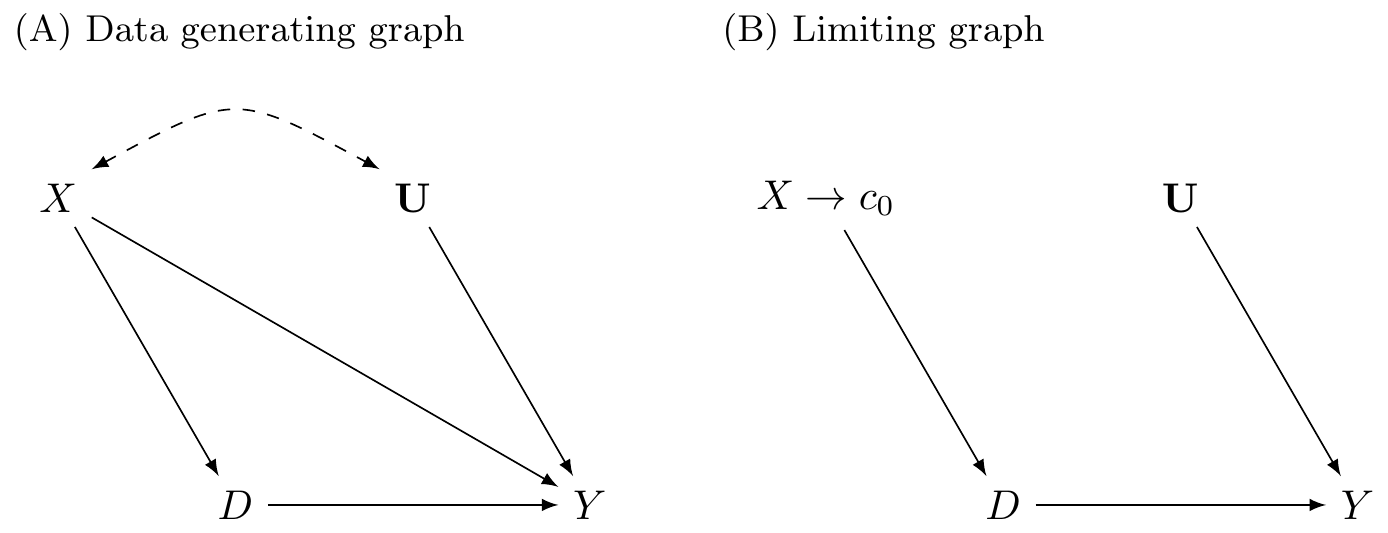
\includegraphics[width=0.7\textwidth]{images/Steiner_DAG_RDD.jpg}
    \captionof{figure}{\textit{DAG for Regression Discontinuity Design \label{fig:Steiner_DAG_RDD} \textcite{steinerGraphicalModelsQuasiexperimental2017}}}
\end{center}

The DAG formalises the causal mechanism causal inference relies on. It is a usaful way to identify possible weakness of the identification strategy. It strenghthen the analysis showing how the effects of treatment on outcome variable is isolated from the effects of confounders.

\vspace*{1em}
In this setting, variables like "Party" and "Competitivness" are confounders. They provide endogenous sources of variation. We take solve this problem controlling for these variables in our regression.

\vspace*{1em}
Omitted variable bias happens when we do not control for all confounders. However, it is impossible to eliminate all sources of endogenous variation because some confounders are not observed. In this instance, the solution is not empirical but qualitative. Therefore, it depends on the knowledge of the context under study.

\subsection{RDD Results}

\begin{center}
    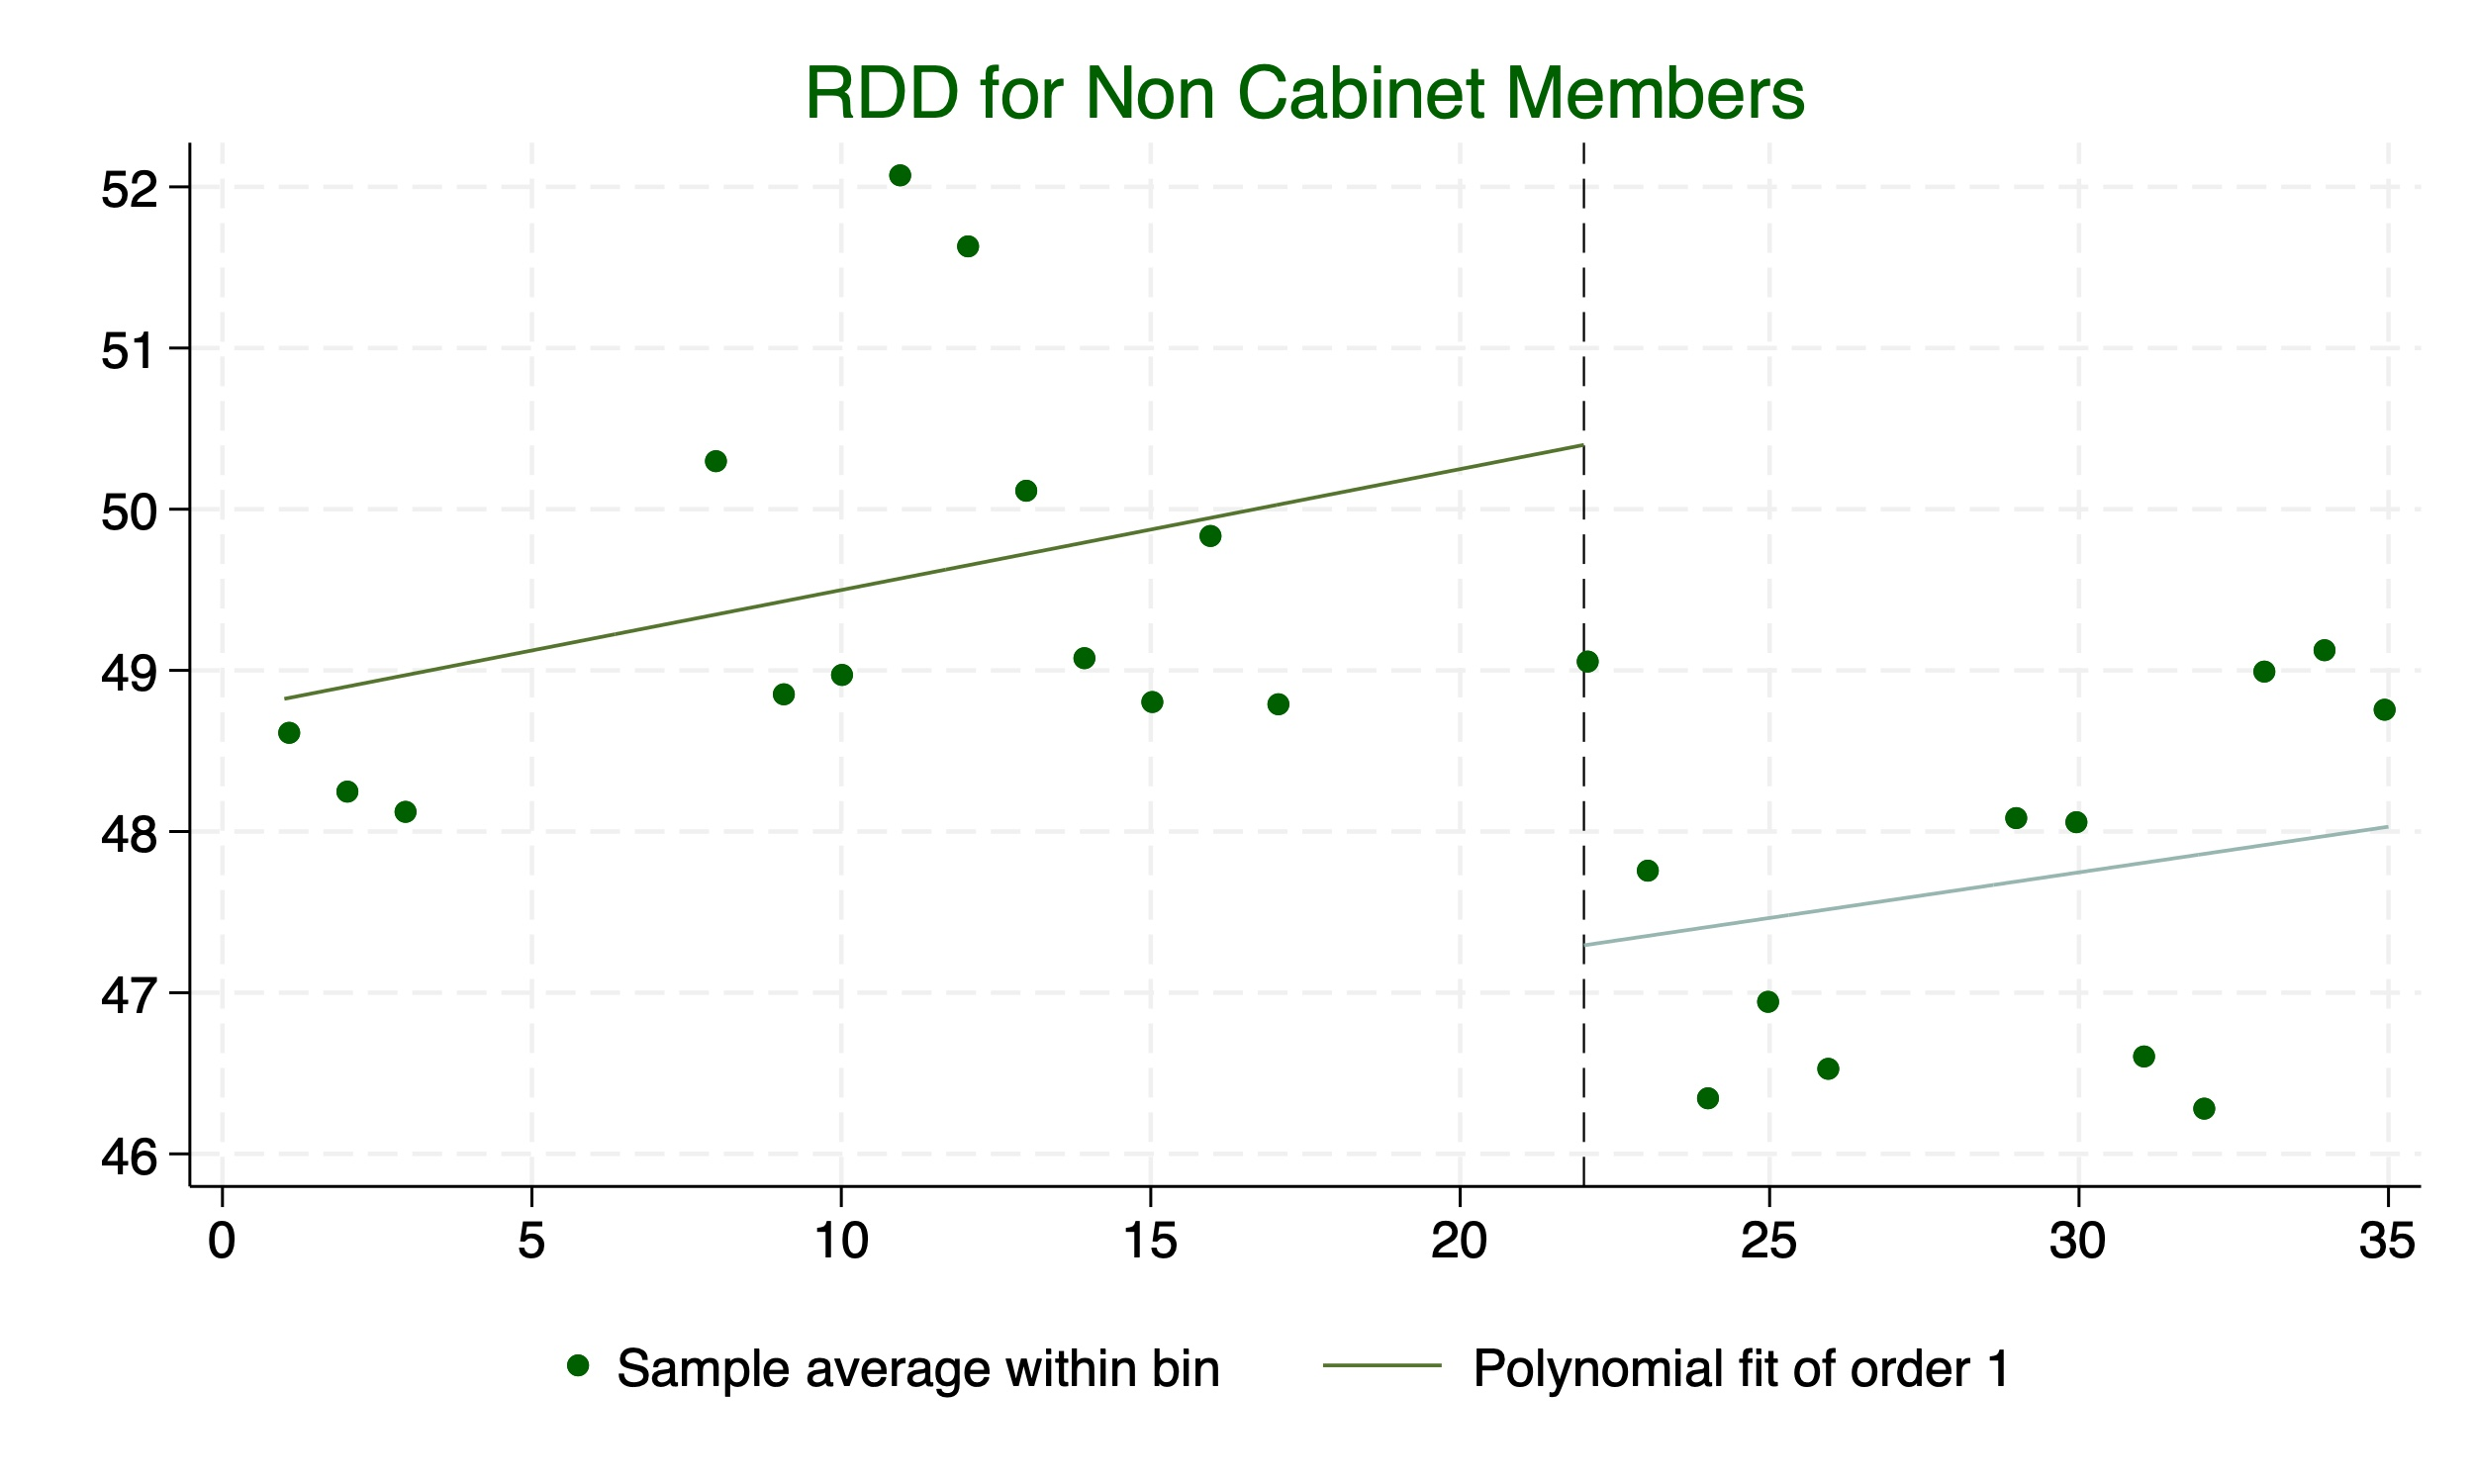
\includegraphics[width=0.7\textwidth]{images/rdplot_fkread_non_cab.jpg}
    \captionof{figure}{\textit{LATE Estimate of RDD for Non Cabinet Members}}
    \label{fig:rdplot_fkread_non_cab}
\end{center}

\begin{center}
    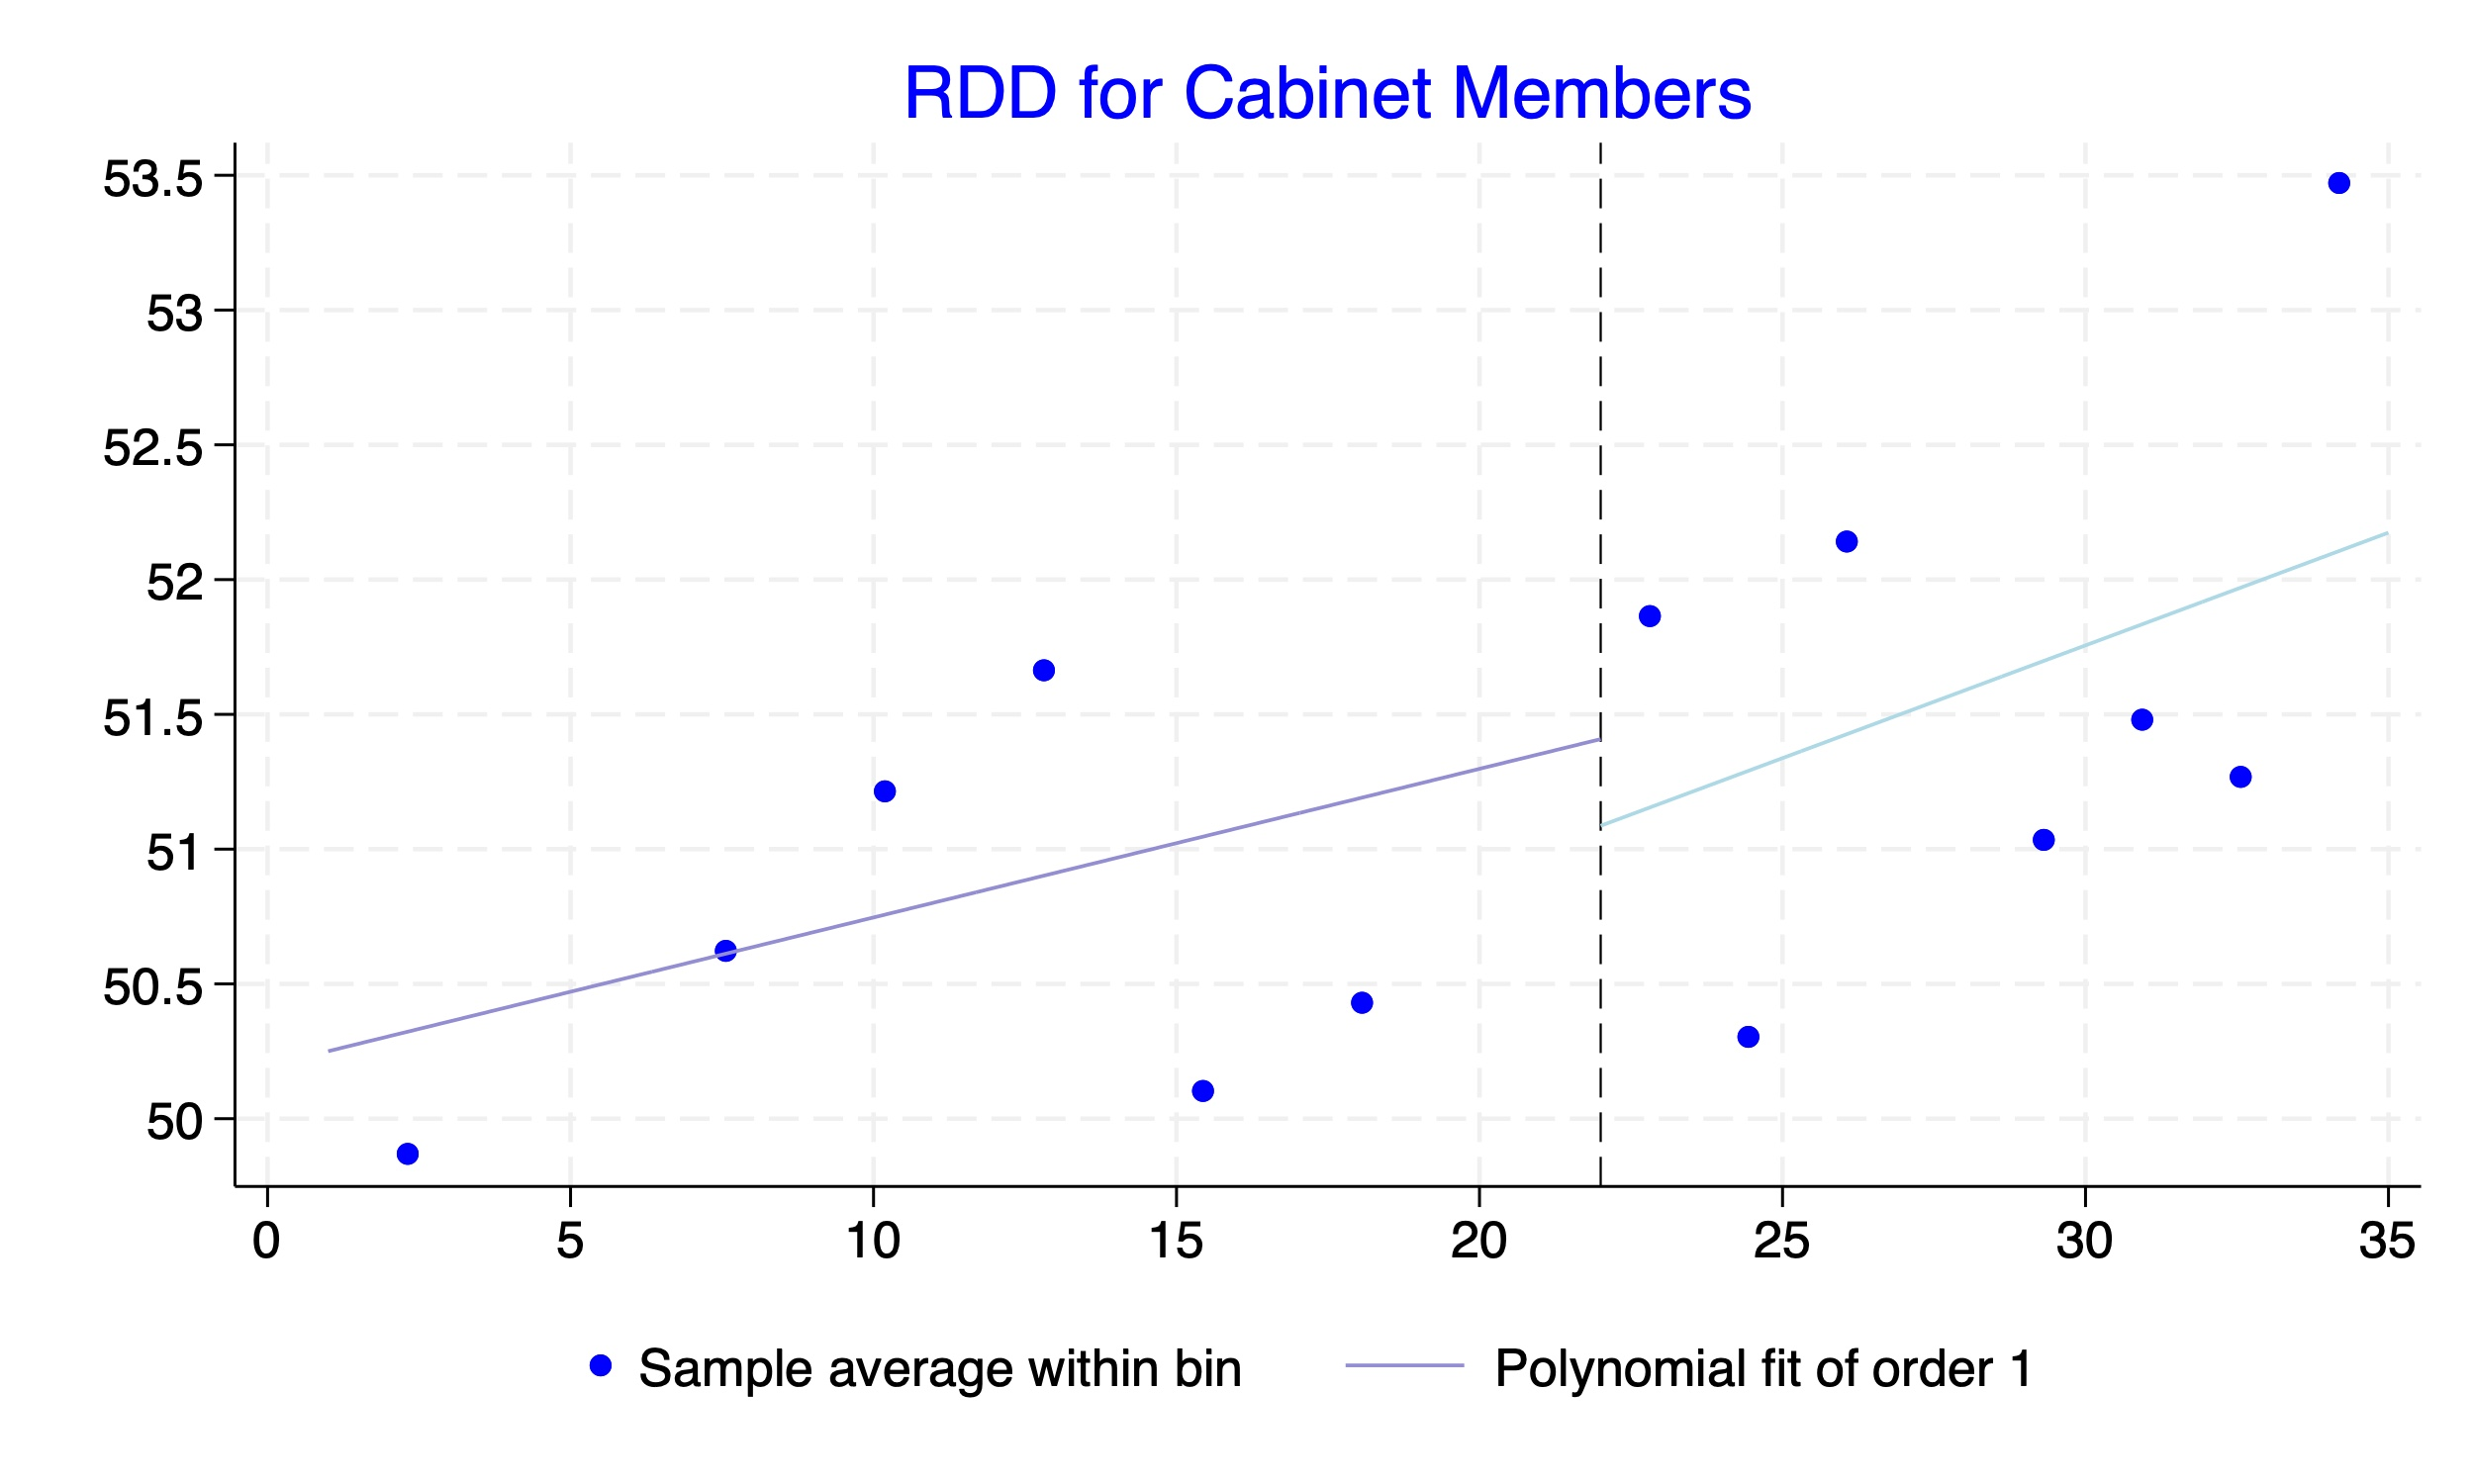
\includegraphics[width=0.7\textwidth]{images/rdplot_fkread.jpg}
    \captionof{figure}{\textit{LATE Estimate of RDD for Cabinet Members}}
    \label{fig:rdplot_fkread}
\end{center}


%------- End of the File -------